% Étape Win : attention dans 16 fenêtres fixes (FreeFlow)
% Compiler avec pdflatex (ou Overleaf).
\documentclass[border=10pt]{standalone}
\usepackage[T1]{fontenc}
\usepackage[utf8]{inputenc}
\usepackage[scaled]{helvet}
\renewcommand{\familydefault}{\sfdefault}
\usepackage{sansmath}
\sansmath
\usepackage{amsmath}
\usepackage{tikz}
\usetikzlibrary{arrows.meta}

% Couleurs du thème
\definecolor{cA}{HTML}{FFE2A8}   % fenêtres : 4 teintes en damier
\definecolor{cB}{HTML}{FFC2C8}
\definecolor{cC}{HTML}{FFB8A0}
\definecolor{cD}{HTML}{F3D6E6}
\definecolor{orange}{HTML}{FFD0BF}
\definecolor{orangeF}{HTML}{F08A6A}
\definecolor{bordeaux}{HTML}{3F161C}
\definecolor{grisclair}{HTML}{F4EEEA}

\tikzset{
  th/.style={font=\fontsize{14}{16}\selectfont\bfseries, text=black, inner sep=0pt},
  ts/.style={font=\fontsize{12}{14}\selectfont, text=black, inner sep=0pt},
  fl/.style={bordeaux, line width=1.5pt, -{Stealth[length=7pt]}},
  lien/.style={bordeaux, line width=0.8pt, dash pattern=on 4pt off 3pt},
}
\newcommand{\num}[1]{\tikz[baseline=(c.base)]\node[circle,draw=black,line width=0.7pt,inner sep=1pt,font=\fontsize{10}{10}\selectfont\bfseries](c){#1};}
% couleur de la fenêtre (ligne de fenêtre a, colonne de fenêtre b) : damier de 4 teintes
\newcommand{\setwin}[2]{%
  \pgfmathtruncatemacro{\idx}{2*mod(#1,2)+mod(#2,2)}%
  \ifcase\idx \def\cc{cA}\or \def\cc{cB}\or \def\cc{cC}\or \def\cc{cD}\fi}

\begin{document}
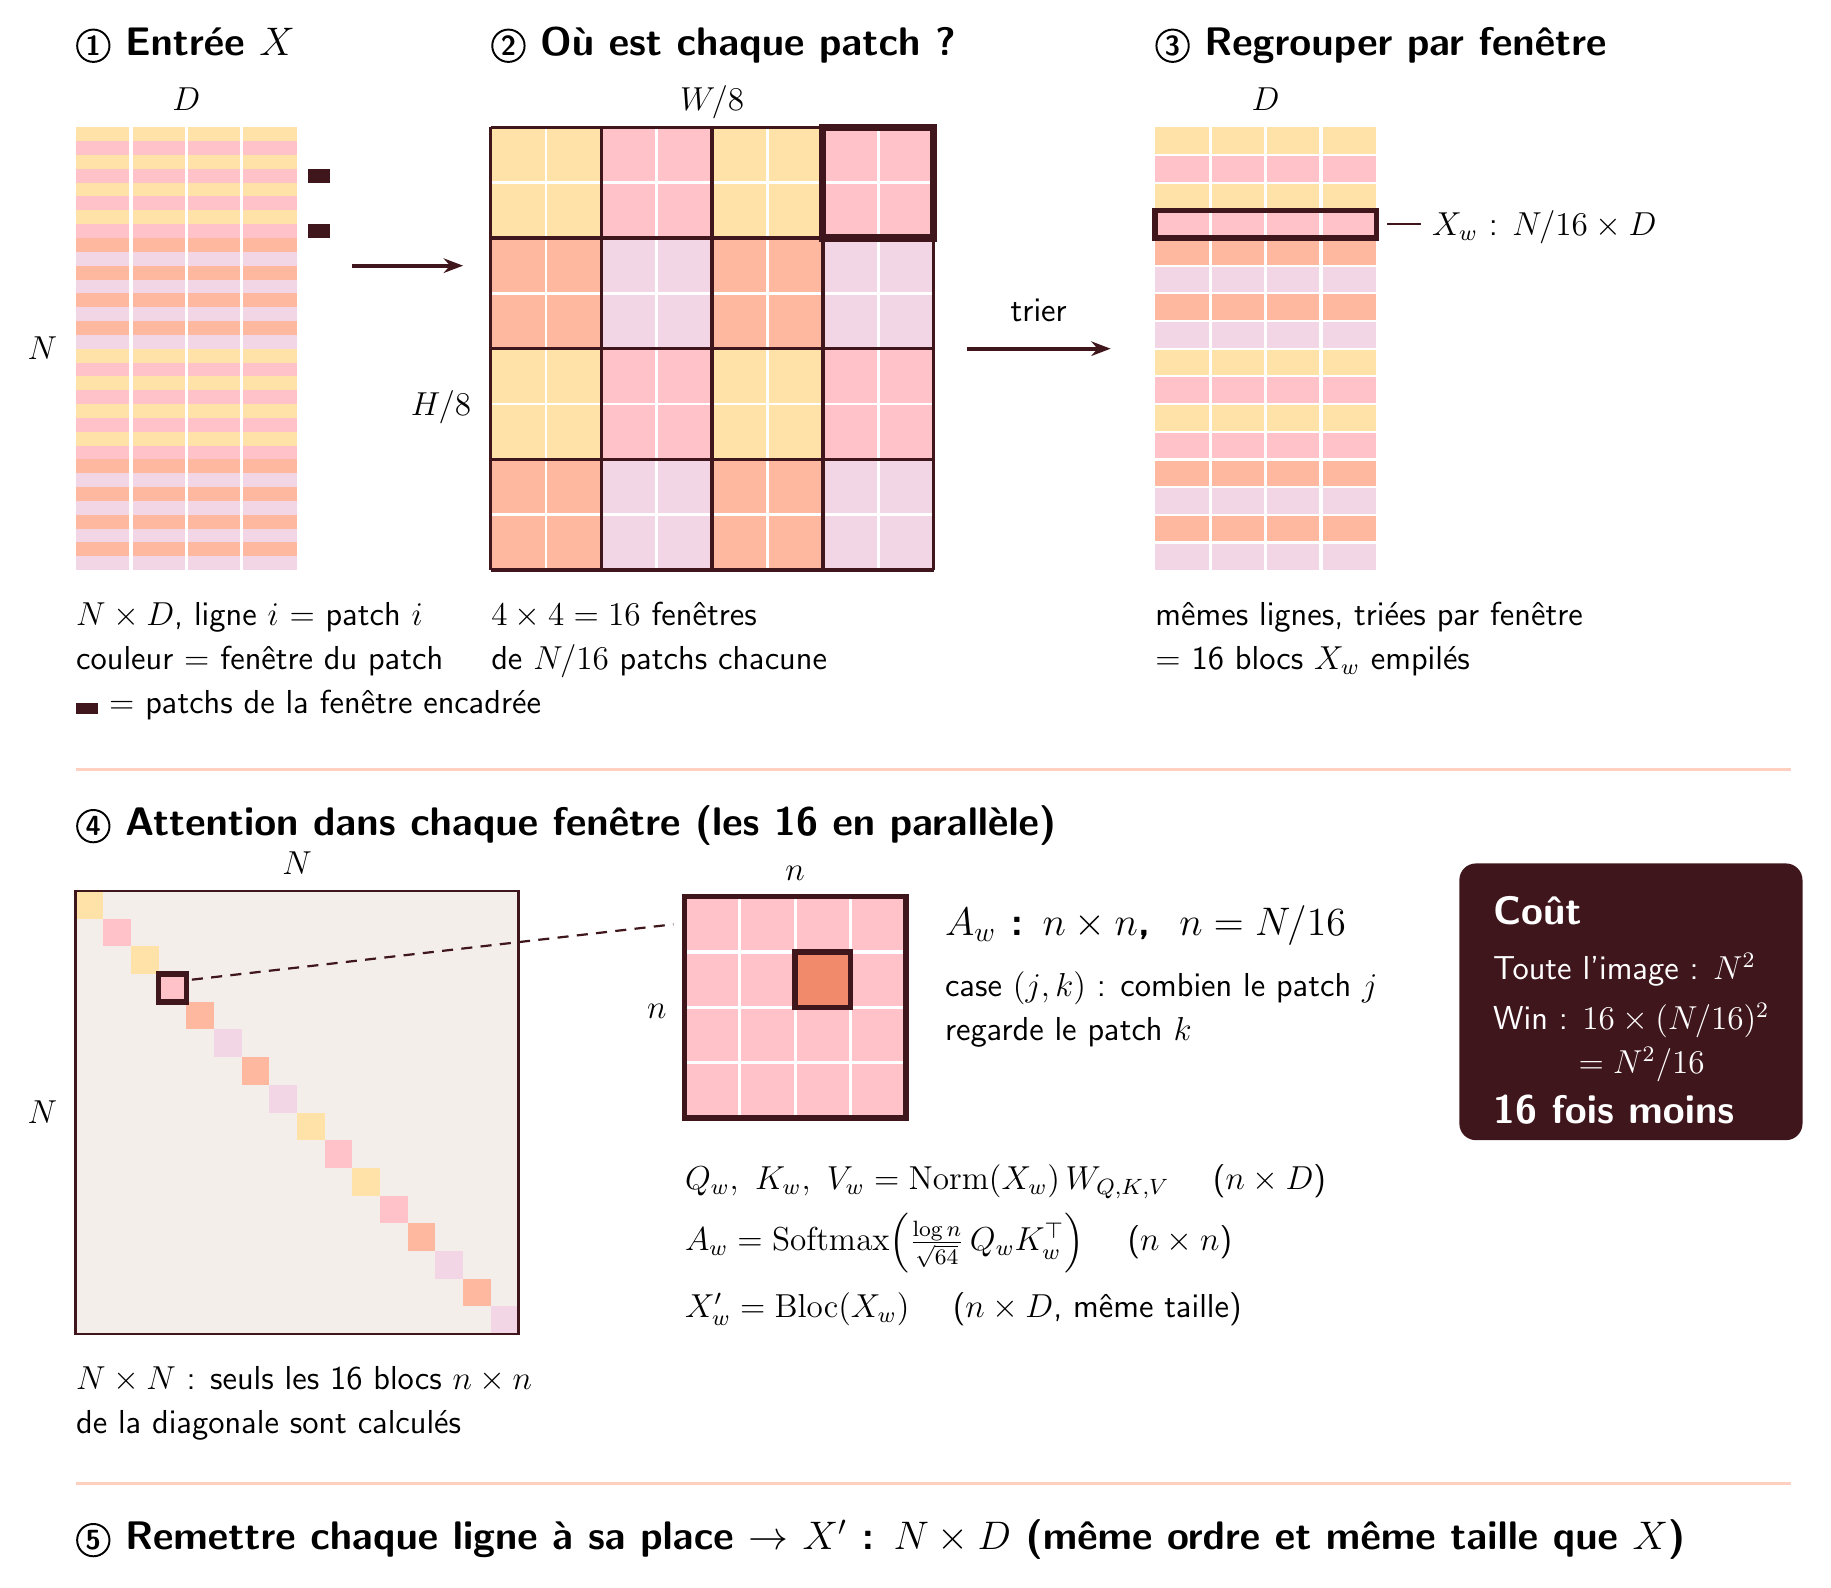
\begin{tikzpicture}[x=1pt, y=-1pt, line join=miter]

% =============== LIGNE 1 ===============
\node[th, anchor=base west] at (40,24)  {\num{1} Entrée $X$};
\node[th, anchor=base west] at (190,24) {\num{2} Où est chaque patch ?};
\node[th, anchor=base west] at (430,24) {\num{3} Regrouper par fenêtre};

% ---- 1. X : N x D, lignes dans l'ordre de l'image (couleur = fenêtre) ----
\foreach \r in {0,...,63} {
  \pgfmathtruncatemacro{\wa}{floor(floor(\r/8)/2)}
  \pgfmathtruncatemacro{\wb}{floor(mod(\r,8)/2)}
  \setwin{\wa}{\wb}
  \fill[\cc] (40,50+2.5*\r) rectangle (120,52.5+2.5*\r);
}
\foreach \x in {60,80,100} \draw[white, line width=1.2pt] (\x,50) -- (\x,210);
\foreach \r in {6,7,14,15} \fill[bordeaux] (124,50+2.5*\r) rectangle (132,52.5+2.5*\r);
\node[ts, anchor=base] at (80,44) {$D$};
\node[ts, anchor=base] at (28,134) {$N$};
\node[ts, anchor=base west] at (40,230) {$N \times D$, ligne $i$ = patch $i$};
\node[ts, anchor=base west] at (40,246) {couleur = fenêtre du patch};

\draw[fl] (140,100) -- (180,100);

% ---- 2. Grille (H/8) x (W/8) : 16 fenêtres ----
\foreach \a in {0,...,7} \foreach \b in {0,...,7} {
  \pgfmathtruncatemacro{\wa}{floor(\a/2)}
  \pgfmathtruncatemacro{\wb}{floor(\b/2)}
  \setwin{\wa}{\wb}
  \filldraw[fill=\cc, draw=white, line width=1pt] (190+20*\b,50+20*\a) rectangle (210+20*\b,70+20*\a);
}
\foreach \k in {0,...,4} {
  \draw[bordeaux, line width=1.2pt] (190+40*\k,50) -- (190+40*\k,210);
  \draw[bordeaux, line width=1.2pt] (190,50+40*\k) -- (350,50+40*\k);
}
\draw[bordeaux, line width=2.6pt] (310,50) rectangle (350,90);
\node[ts, anchor=base] at (270,44) {$W/8$};
\node[ts, anchor=base] at (172,154) {$H/8$};
\node[ts, anchor=base west] at (190,230) {$4 \times 4 = 16$ fenêtres};
\node[ts, anchor=base west] at (190,246) {de $N/16$ patchs chacune};

\draw[fl] (362,130) -- (414,130);
\node[ts, anchor=base] at (388,120) {trier};

% ---- 3. X~ : mêmes lignes triées par fenêtre = 16 blocs X_w ----
\foreach \k in {0,...,15} {
  \pgfmathtruncatemacro{\wa}{floor(\k/4)}
  \pgfmathtruncatemacro{\wb}{mod(\k,4)}
  \setwin{\wa}{\wb}
  \fill[\cc] (430,50+10*\k) rectangle (510,60+10*\k);
}
\foreach \x in {450,470,490} \draw[white, line width=1.2pt] (\x,50) -- (\x,210);
\foreach \k in {1,...,15} \draw[white, line width=0.8pt] (430,50+10*\k) -- (510,50+10*\k);
\draw[bordeaux, line width=2pt] (430,80) rectangle (510,90);
\node[ts, anchor=base] at (470,44) {$D$};
\draw[bordeaux, line width=0.8pt] (514,85) -- (526,85);
\node[ts, anchor=base west] at (530,89) {$X_w$ : $N/16 \times D$};
\node[ts, anchor=base west] at (430,230) {mêmes lignes, triées par fenêtre};
\node[ts, anchor=base west] at (430,246) {$=$ 16 blocs $X_w$ empilés};

\node[ts, anchor=base west] at (40,262) {\textcolor{bordeaux}{\rule{8pt}{4pt}} = patchs de la fenêtre encadrée};
\begin{scope}[yshift=-16pt]
% =============== LIGNE 2 ===============
\draw[orange, line width=1pt] (40,266) -- (660,266);
\node[th, anchor=base west] at (40,290) {\num{4} Attention dans chaque fenêtre (les 16 en parallèle)};

% ---- matrice N x N : blocs diagonaux seulement ----
\fill[grisclair] (40,310) rectangle (200,470);
\foreach \k in {0,...,15} {
  \pgfmathtruncatemacro{\wa}{floor(\k/4)}
  \pgfmathtruncatemacro{\wb}{mod(\k,4)}
  \setwin{\wa}{\wb}
  \fill[\cc] (40+10*\k,310+10*\k) rectangle (50+10*\k,320+10*\k);
}
\draw[bordeaux, line width=1pt] (40,310) rectangle (200,470);
\draw[bordeaux, line width=2pt] (70,340) rectangle (80,350);
\node[ts, anchor=base] at (120,304) {$N$};
\node[ts, anchor=base] at (28,394) {$N$};
\node[ts, anchor=base west] at (40,490) {$N \times N$ : seuls les 16 blocs $n \times n$};
\node[ts, anchor=base west] at (40,506) {de la diagonale sont calculés};

\draw[lien] (82,342) -- (256,322);

% ---- zoom : A_w (n x n) ----
\foreach \j in {0,...,3} \foreach \k in {0,...,3}
  \filldraw[fill=cB, draw=white, line width=1.2pt] (260+20*\k,312+20*\j) rectangle (280+20*\k,332+20*\j);
\filldraw[fill=orangeF, draw=bordeaux, line width=2pt] (300,332) rectangle (320,352);
\draw[bordeaux, line width=2pt] (260,312) rectangle (340,392);
\node[ts, anchor=base] at (300,306) {$n$};
\node[ts, anchor=base] at (250,356) {$n$};
\node[th, anchor=base west] at (354,326) {$A_w$ : $n \times n$, \ $n = N/16$};
\node[ts, anchor=base west] at (354,348) {case $(j,k)$ : combien le patch $j$};
\node[ts, anchor=base west] at (354,364) {regarde le patch $k$};

\node[ts, anchor=base west] at (260,418) {$Q_w,\ K_w,\ V_w = \mathrm{Norm}(X_w)\, W_{Q,K,V}$ \quad ($n \times D$)};
\node[ts, anchor=base west] at (260,440) {$A_w = \mathrm{Softmax}\!\left(\frac{\log n}{\sqrt{64}}\, Q_w K_w^{\top}\right)$ \quad ($n \times n$)};
\node[ts, anchor=base west] at (260,464) {$X'_w = \mathrm{Bloc}(X_w)$ \quad ($n \times D$, même taille)};

% ---- coût ----
\filldraw[fill=bordeaux, draw=none, rounded corners=6pt] (540,300) rectangle (664,400);
\node[th, anchor=base west, text=white] at (552,322) {Coût};
\node[ts, anchor=base west, text=white] at (552,342) {Toute l'image : $N^2$};
\node[ts, anchor=base west, text=white] at (552,360) {Win : $16 \times (N/16)^2$};
\node[ts, anchor=base west, text=white] at (552,376) {\phantom{Win :} $= N^2/16$};
\node[th, anchor=base west, text=white] at (552,394) {16 fois moins};

% =============== LIGNE 3 ===============
\draw[orange, line width=1pt] (40,524) -- (660,524);
\node[th, anchor=base west] at (40,548) {\num{5} Remettre chaque ligne à sa place $\rightarrow$ $X'$ : $N \times D$ (même ordre et même taille que $X$)};

\end{scope}
\end{tikzpicture}
\end{document}
